% Appendix C

\chapter{Project Management} % Main appendix title

\label{AppendixC} % For referencing this appendix elsewhere, use \ref{AppendixA}

\lhead{Appendix C. \emph{Appendix C}} % This is for the header on each page - perhaps a shortened title

\section{Risk Management}
\label{risman}

The list of expected risks and proposed mitigations is given in Table \ref{risktab}. As explained in the table, there are three main risks: having longer than expected training times, being incapable of replicating experimental results and having compatibility issues on my Ubuntu ARM64 VM. The primary approach to minimising those risks will be to prioritise the most complicated aspects of the project; some of that work was done in the preliminary investigations, as explained in Section \ref{preli}. This will let me identify problems early in the process, and I will be able to ask for help and advice before I run out of time.

\begin{table}
\centering
\begin{tabularx}{\textwidth}{||X|X|X|X||} 
 \hline
 Risk & Likelihood & Impact & Mitigation\\ [0.5ex] 
 \hline\hline
 Unable to replicate results of \cite{bosello} and \cite{Reference4} & Medium & High & Allocate highest priority to task in the project plan; ask supervisor for advice\\
 \hline
  Involuntary plagiarism by missing something in the wider literature & Low & High & Do regular literature reviews on specific points; ask supervisor for input\\
  
  \hline
  Training the RL controllers takes longer than expected & High & Medium & Optimise the code, reduce the size of NNs, use other hardware, possibly Cloud computing or Google Colab\\ [1ex]

 \hline
  Loss of Python and/or \LaTeX $ $ files due to hardware failure or human error& Low & High & Save files regularly on the Cloud or an external drive\\ [1ex]
 
   \hline
  Compatibility errors with ML Python libraries on my Ubuntu ARM64 VM setup & Medium & High & Ask for help on StackOverflow, use different machine or libraries if necessary\\
  
   \hline
  Tuning manually the PID parameters $K_p$, $K_i$ and $K_d$ for the Wall Following controller doesn't work & Medium & Medium & Use MATLAB or possibly the ROS \verb |pid| package\\
  
 \hline
    Applying the controllers on the physical car doesn't work: it damages the car, there are delays in communications with the actuators and sensors, the LiDAR data is not as perfect as in the simulator & Medium & High & Increase speed progressively, implement a safety module in the ROS code to stop the car if it gets too close to a wall, make sure the walls of the track are not made out of reflective materials\\ [1ex]
   
 \hline
 
\end{tabularx}
\caption{Risk assessment approach}
\label{risktab}
\end{table}


\section{Project Plan}
\label{propla}

The GANT chart introduces the project plan (Figure \ref{gantt}). Because I don't have any constraints related to equipment availability or human evaluations, I was able to plan everything around my own constraints, especially the time needed to train the controllers for DQN and DDPG. \\

\begin{landscape}
\phantom{centering}\\
\phantom{centering}\\
\phantom{centering}\\
\begin{figure}[H]
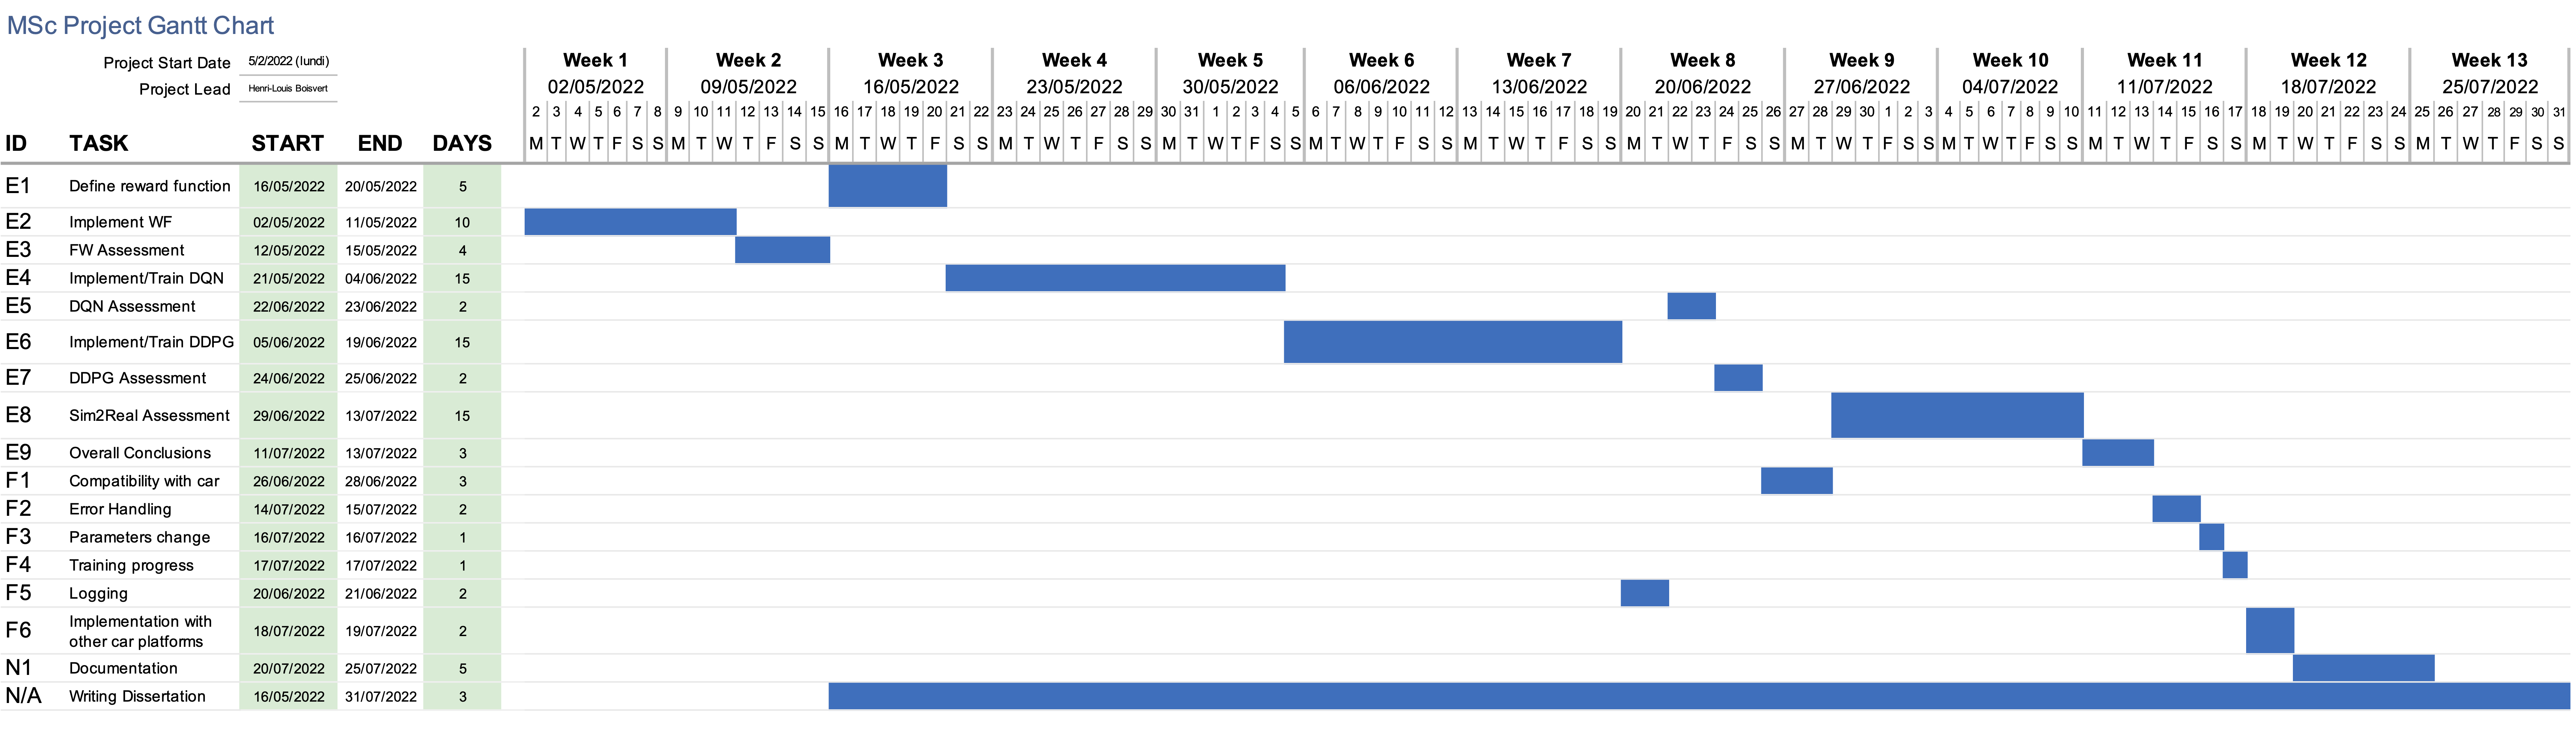
\includegraphics[angle=0, scale=0.092]{Figures/gantt.png}
\caption{Gantt Chart of the project}
\label{gantt}
\end{figure}
\end{landscape}